\begin{frame}
    \frametitle{\problemtitle}
    \begin{block}{Problem}
	  Given $2n$ points, is there a point that occurs an odd number of times?
	\end{block}
	\pause
	\begin{block}{Solutions}
	  \begin{itemize}
	    \item Sort the points, check whether point $2i-1$ equals point $2i$ in $\mathcal O(n \log n)$
	    \item XOR hashes of all points in $\mathcal{O}(n)$
	  \end{itemize}
	\end{block}
\end{frame}

\begin{frame}
    \frametitle{\problemtitle}
    \begin{block}{Problem}
      Given $n\leq 1000$ line segments that partition the plane in small
      regions.
      Are there two regions the same \emph{distance} from the ocean?
    \end{block}
    \pause
    \begin{block}{Geometry solution}
      Find all intersections and construct the dual graph on faces:\\
      Costs $\mathcal{O}\left(n^2\log n\right)$ and your sanity ($256$ lines of C++).
    \end{block}
\end{frame}
\begin{frame}
    \frametitle{\problemtitle}
    \begin{block}{Problem}
      Given $n\leq 1000$ line segments that partition the plane in small
      regions.
      Are there two regions the same \emph{distance} from the ocean?
    \end{block}
    \begin{block}{Intended solution}
      \begin{columns}
      \begin{column}{0.5\textwidth}
      \begin{itemize}
        \item<+-> Consider the dual graph, with one vertex per region.
        \item<+-> The answer is \texttt{yes} if there are adjacent regions with equal distance to the ocean.
        \item<+-> The difference between adjacent distances is at most $1$, so we can work modulo $2$ instead.
        \item<+-> The answer is \texttt{no} iff all pairs of adjacent faces have
          opposite values.
      \end{itemize}
      \end{column}
      \begin{column}{0.42\textwidth}
      \begin{center}
      \only<-2>{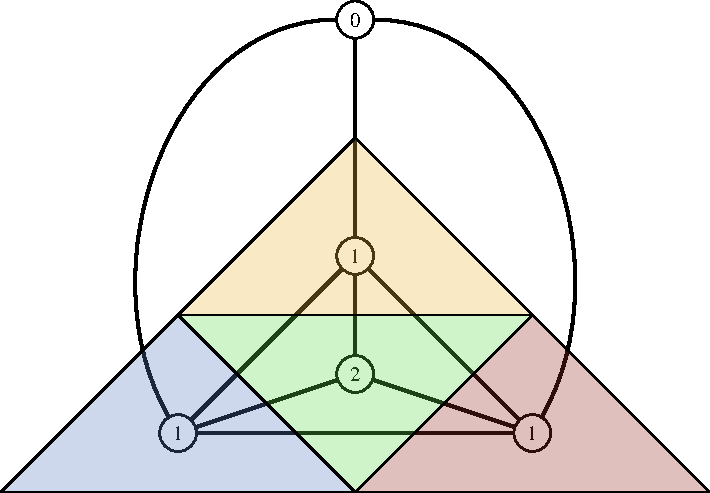
\includegraphics[scale=0.4]{sample2-graph.pdf}}%
      \only<3->{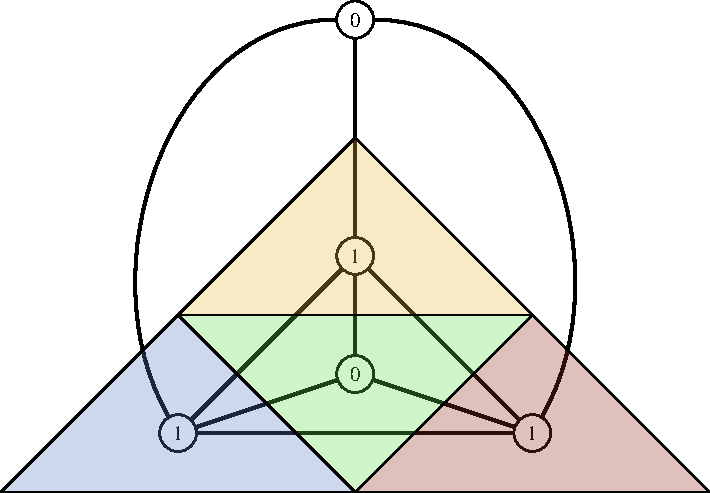
\includegraphics[scale=0.4]{sample2-graph-mod2.pdf}}%
      \end{center}
      \end{column}
      \end{columns}
    \end{block}
\end{frame}
\begin{frame}
    \frametitle{\problemtitle}
    \begin{block}{Problem}
      Given $n\leq 1000$ line segments that partition the plane in small
      regions.
      Are there two regions the same \emph{distance} from the ocean?
    \end{block}
    \begin{block}{Intended solution}
      \begin{columns}
      \begin{column}{0.5\textwidth}
      \begin{itemize}
        \item<+-> The answer is \texttt{no} iff all pairs of adjacent faces have
          opposite values.
        \item<+-> I.e.: the dual graph must be bipartite.
        \item<+-> That's true iff in each intersection point an even number of
          lines meet.
        \item<+-> Solution: check if each segment endpoint appears an even number of
          times in the input.
      \end{itemize}
      \end{column}
      \begin{column}{0.42\textwidth}
      \begin{center}
      \only<1>{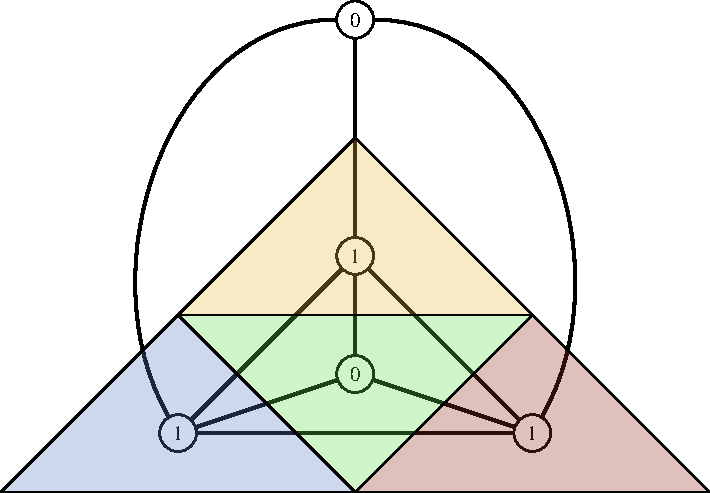
\includegraphics[scale=0.4]{sample2-graph-mod2.pdf}}%
      \only<2->{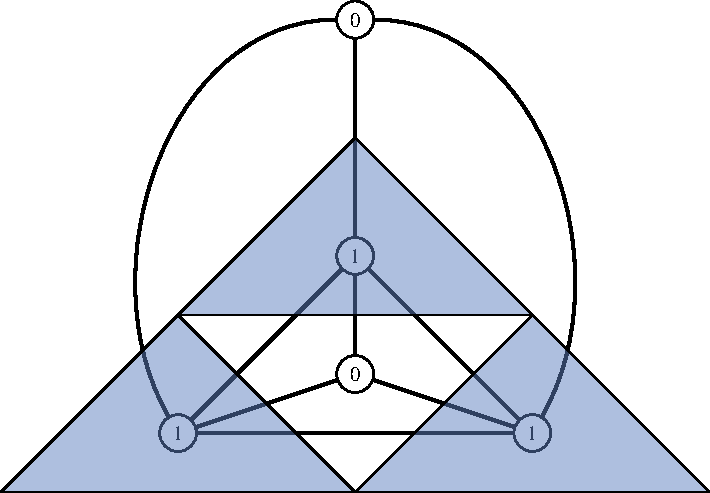
\includegraphics[scale=0.4]{sample2-graph-bipartite.pdf}}%
      \end{center}
      \end{column}
      \end{columns}
    \end{block}
    \solvestats
\end{frame}

\begin{frame}
    \frametitle{\problemtitle}
    \centering
    \includegraphics<+>[height=0.8\textheight]{vis-1}%
    \includegraphics<+>[height=0.8\textheight]{vis-2}%
    \includegraphics<+>[height=0.8\textheight]{vis-3}%
\end{frame}
